\documentclass[8pt]{beamer}

\newif\ifplacelogo % create a new conditional
\placelogotrue % set it to true

\usetheme{Warsaw}
\usecolortheme{rose}
\usepackage{multicol}
\usepackage{epstopdf}
\usepackage[italic]{hepnames}
\usepackage{tikz}
\usepackage{listings}
\usepackage{times}
\usepackage{amsmath}
\usepackage{verbatim}
\usepackage{hyperref}
\usepackage{bbding}
\lstset{breakatwhitespace,
language=C++,
columns=fullflexible,
keepspaces,
breaklines,
tabsize=3, 
showstringspaces=false,
extendedchars=true}

% TikZ includes!!!
\usepackage{tikz}
\usetikzlibrary{backgrounds}
\usetikzlibrary{calc}
\tikzstyle{every picture}+=[remember picture]
\input{/home/oviazlo/Desktop/beamerPresentations/myReports/latexHelpScripts/tikzGrid.tex}


\begin{document}

% custom colors
\definecolor{olive}{rgb}{0.3, 0.4, .1}
\definecolor{fore}{RGB}{249,242,215}
\definecolor{back}{RGB}{51,51,51}
\definecolor{title}{RGB}{255,0,90}
\definecolor{dgreen}{rgb}{0.,0.6,0.}
\definecolor{gold}{rgb}{1.,0.84,0.}
\definecolor{JungleGreen}{cmyk}{0.99,0,0.52,0}
\definecolor{BlueGreen}{cmyk}{0.85,0,0.33,0}
\definecolor{RawSienna}{cmyk}{0,0.72,1,0.45}
\definecolor{Magenta}{cmyk}{0,1,0,0}

\definecolor{PixelColor}{RGB}{207,232,139}
\definecolor{SCTColor}{RGB}{167,166,255}
\definecolor{TRTColor}{RGB}{250,224,140}
\definecolor{grayColor}{RGB}{153,153,153}

\newcommand{\yRefPosOne}{0.0}
\newcommand{\xRefPosOne}{0.0}
\newcommand{\yRefPosTwo}{0.0}
\newcommand{\xRefPosTwo}{0.0}
\newcommand{\yRefIncrementOne}{0.0}
\newcommand{\xRefIncrementOne}{0.0}
\newcommand{\yRefIncrementTwo}{0.0}
\newcommand{\xRefIncrementTwo}{0.0}

\graphicspath{ {/home/oviazlo/Desktop/beamerPresentations/FCCee/pictures/plots_oct25_2017/} }
\DeclareGraphicsExtensions{.eps, .pdf, .png}

\newcommand{\myBox}[2][pink] {
    \noindent\colorbox{#1}{
	\textbf{#2}
    }\par
}

% For nice block (provided by Oleh)
\tikzstyle{mybox} = [draw=red, fill=blue!1, very thick,
    rectangle, rounded corners, inner sep=5pt, inner ysep=9pt]
\tikzstyle{fancytitle} =[fill=white!15, text=black]
    
\tikzstyle{PixelBox} = [draw=PixelColor, fill=blue!1, very thick,
    rectangle, rounded corners, inner sep=5pt, inner ysep=9pt]
\tikzstyle{SCTBox} = [draw=SCTColor, fill=blue!1, very thick,
    rectangle, rounded corners, inner sep=5pt, inner ysep=9pt]
\tikzstyle{TRTBox} = [draw=TRTColor, fill=blue!1, very thick,
    rectangle, rounded corners, inner sep=5pt, inner ysep=9pt]

% poster advertisement
\newcommand{\myCenterBox}[2][pink] {
   {\centering
    \noindent\colorbox{#1}{
	\textbf{#2}
    }\par
  }
}

\newcommand{\mySmallCenterBox}[2][pink] {
   {\centering
    \noindent\colorbox{#1}{
	\textbf{{\small #2}}
    }\par
  }
}

\newcommand{\myVerySmallCenterBox}[2][pink] {
   {\centering
    \noindent\colorbox{#1}{
	\textbf{{\scriptsize #2}}
    }\par
  }
}

\newcommand{\backupbegin}{
   \newcounter{finalframe}
   \setcounter{finalframe}{\value{framenumber}}
}
\newcommand{\backupend}{
   \setcounter{framenumber}{\value{finalframe}}
}

\newcommand{\myNode}{\tikz[baseline,inner sep=1pt] \node[anchor=base]}

\definecolor{light-gray}{gray}{0.95}
% poster advertisement


\title[ Calorimeter performance studies \hspace{13.5em}\insertframenumber/
\inserttotalframenumber]{ Calorimeter performance studies }


	\author[Oleksandr Viazlo]{Oleksandr Viazlo \\ 
% 	{\small ???}
	}
	\institute{\small FCC-ee MDI study group meeting\\} 
	
       
	\date{18 October 2017}

% 	\logo{ \ifplacelogo \includegraphics[height=1.8cm]{./ID_week2/lund_uni-logo_s.pdf} \hspace{0.4cm} \fi}

	
   	\frame{\titlepage}

   	

\placelogofalse

%*****************************************************************************
\begin{frame}{\large \large Introduction}
 
\renewcommand{\yRefPosOne}{0.4}
\renewcommand{\xRefPosOne}{2.5}
\renewcommand{\xRefIncrementOne}{5.5}
\begin{tikzpicture}[overlay]


\node [PixelBox] at (\xRefPosOne+2.5,\yRefPosOne+1) (box){%
  \begin{minipage}{\textwidth}
    \begin{itemize}
      \item Charged particle efficiency in the transition region with new iLCSoft release 2017-10-20
      \item Jet energy resolution with FCC-ee vs CLIC detectors
    \end{itemize}
  \end{minipage}
};
\node[fancytitle, right=15pt] at (box.north west) {Content};

\node [TRTBox] at (\xRefPosOne+2.5,\yRefPosOne-2.5) (box){%
    \begin{minipage}{\textwidth}
%        \scriptsize 
        \begin{itemize}
      \item Pandora reconstructed types: $\mu$-, $\pi$-, $e$-, $\gamma$ and neutron 
      \item Efficiency defined as: \\ \vspace{0.1cm}
      \begin{itemize}
       \item denominator: number of truth particles produced on generator level
       \item numerator: number of PFOs with properly reconstructed type (consider only most energetic PFO in the event) 
      \end{itemize}
    \end{itemize}

    \end{minipage}
};
\node[fancytitle, right=15pt] at (box.north west) {Reminder};

\end{tikzpicture}

  
\end{frame}
%*****************************************************************************

%*****************************************************************************
\begin{frame}{\large \large Single charged particle ID efficiency}
% TODO change legend for electron plot. ``Nominal'' -> ``Default Pandora''

\renewcommand{\yRefPosOne}{0}
\renewcommand{\xRefPosOne}{5.3}
\renewcommand{\xRefIncrementOne}{5.5}
\begin{tikzpicture}[overlay]

 \node[inner sep=0pt] (tmp) at (\xRefPosOne-3,\yRefPosOne+1.5)
    {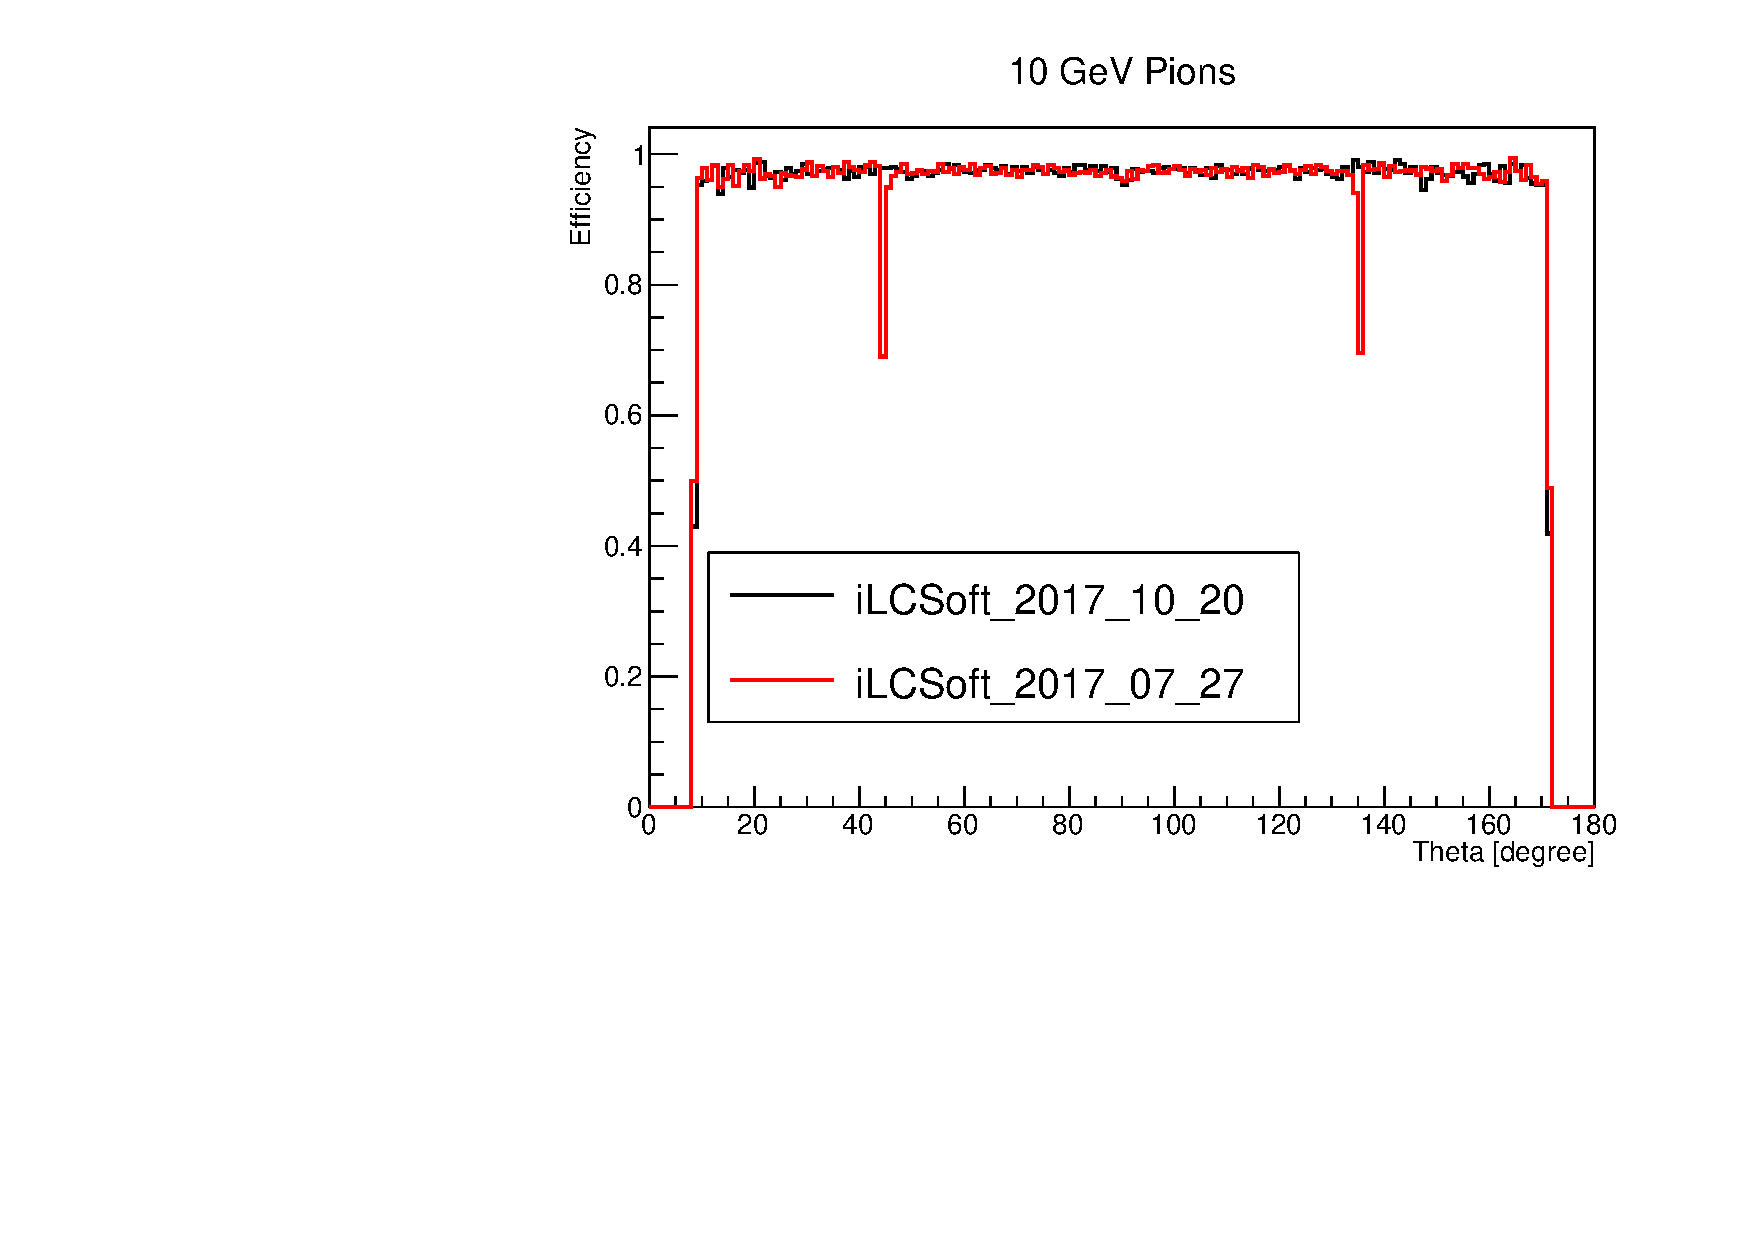
\includegraphics[width=6cm]{pions_eff_vs_theta.pdf}};
  \node [Box] at (\xRefPosOne-3,\yRefPosOne+3.5) (box){%
    \myCenterBox{10 GeV Pions}
  };

 \node[inner sep=0pt] (tmp) at (\xRefPosOne+3,\yRefPosOne+1.5)
    {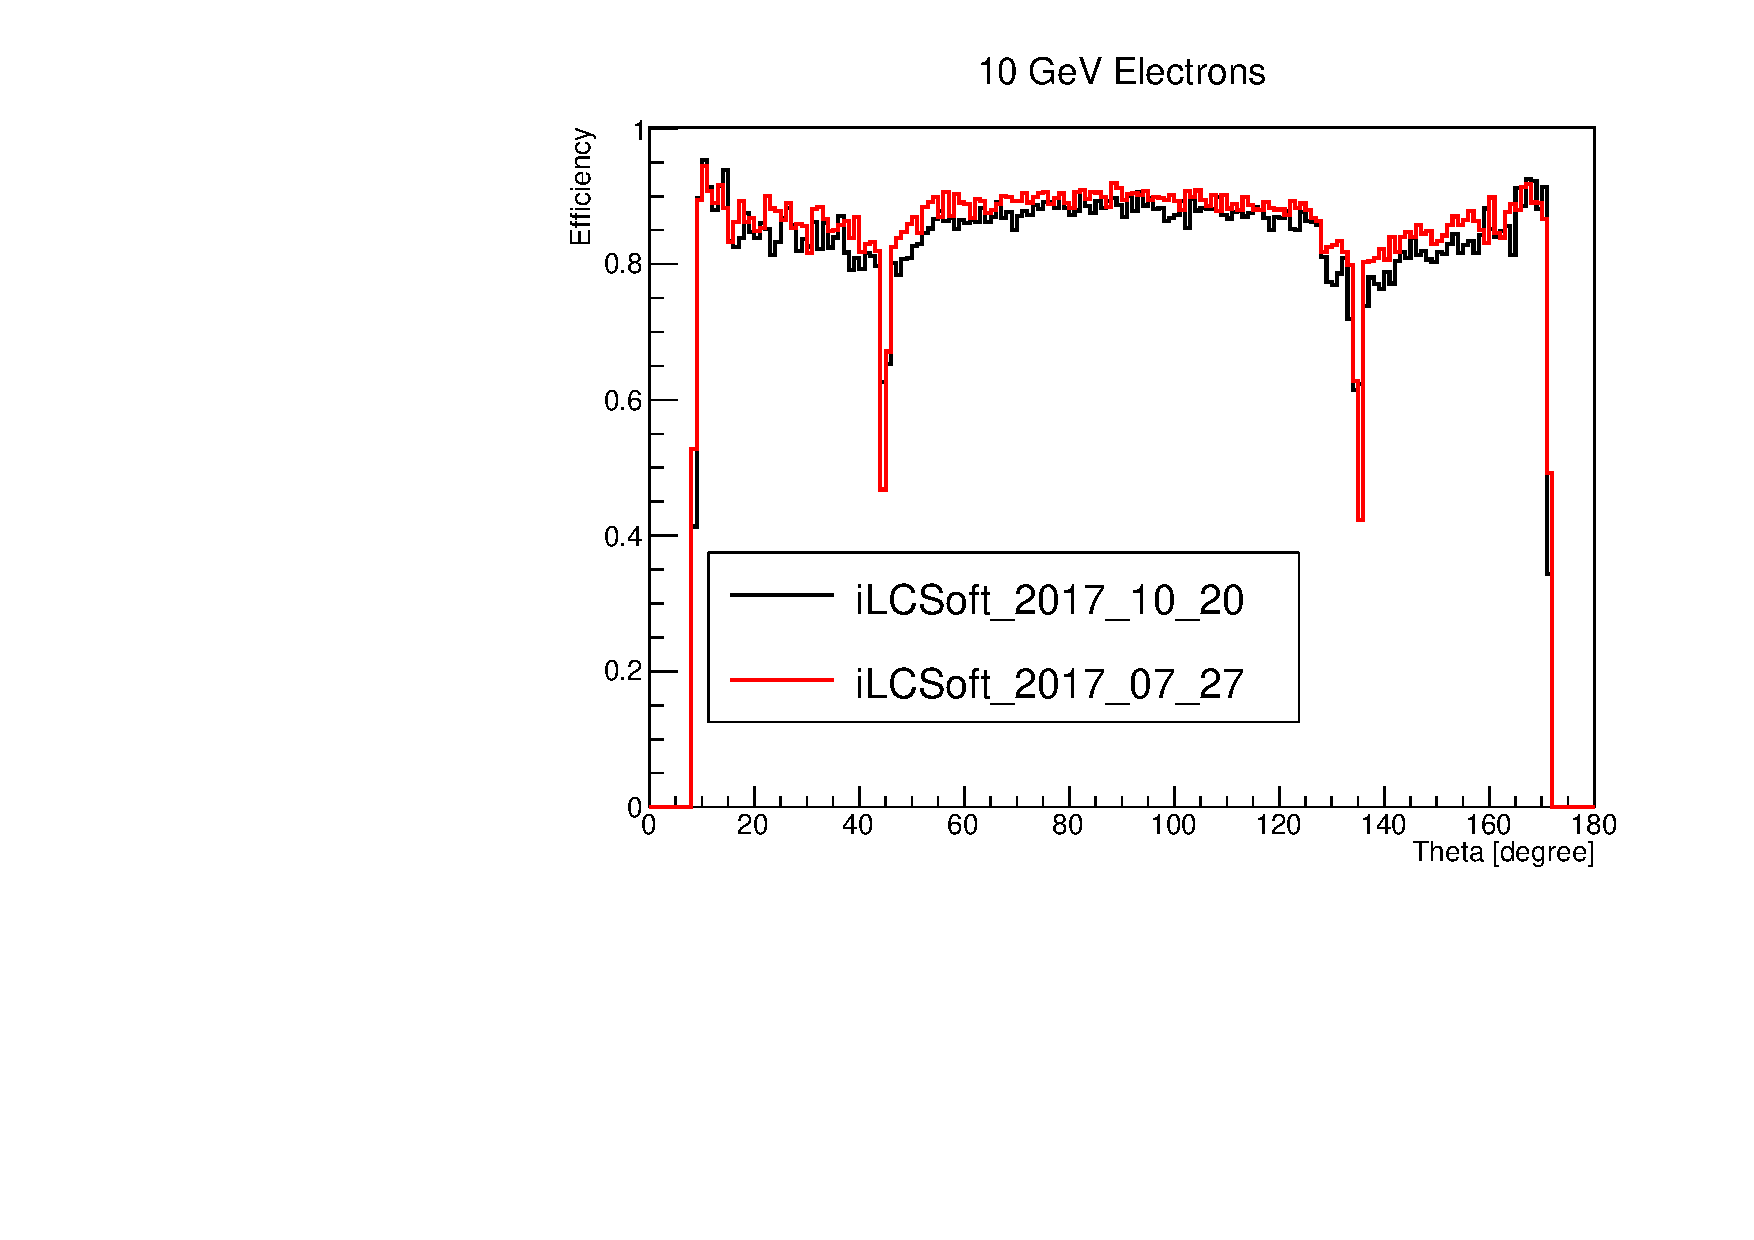
\includegraphics[width=6cm]{electrons_eff_vs_theta.pdf}};
  \node [Box] at (\xRefPosOne+3,\yRefPosOne+3.5) (box){%
    \myCenterBox{10 GeV Electrons}
  };

 \node[inner sep=0pt] (tmp) at (\xRefPosOne+3,\yRefPosOne-2.7)
    {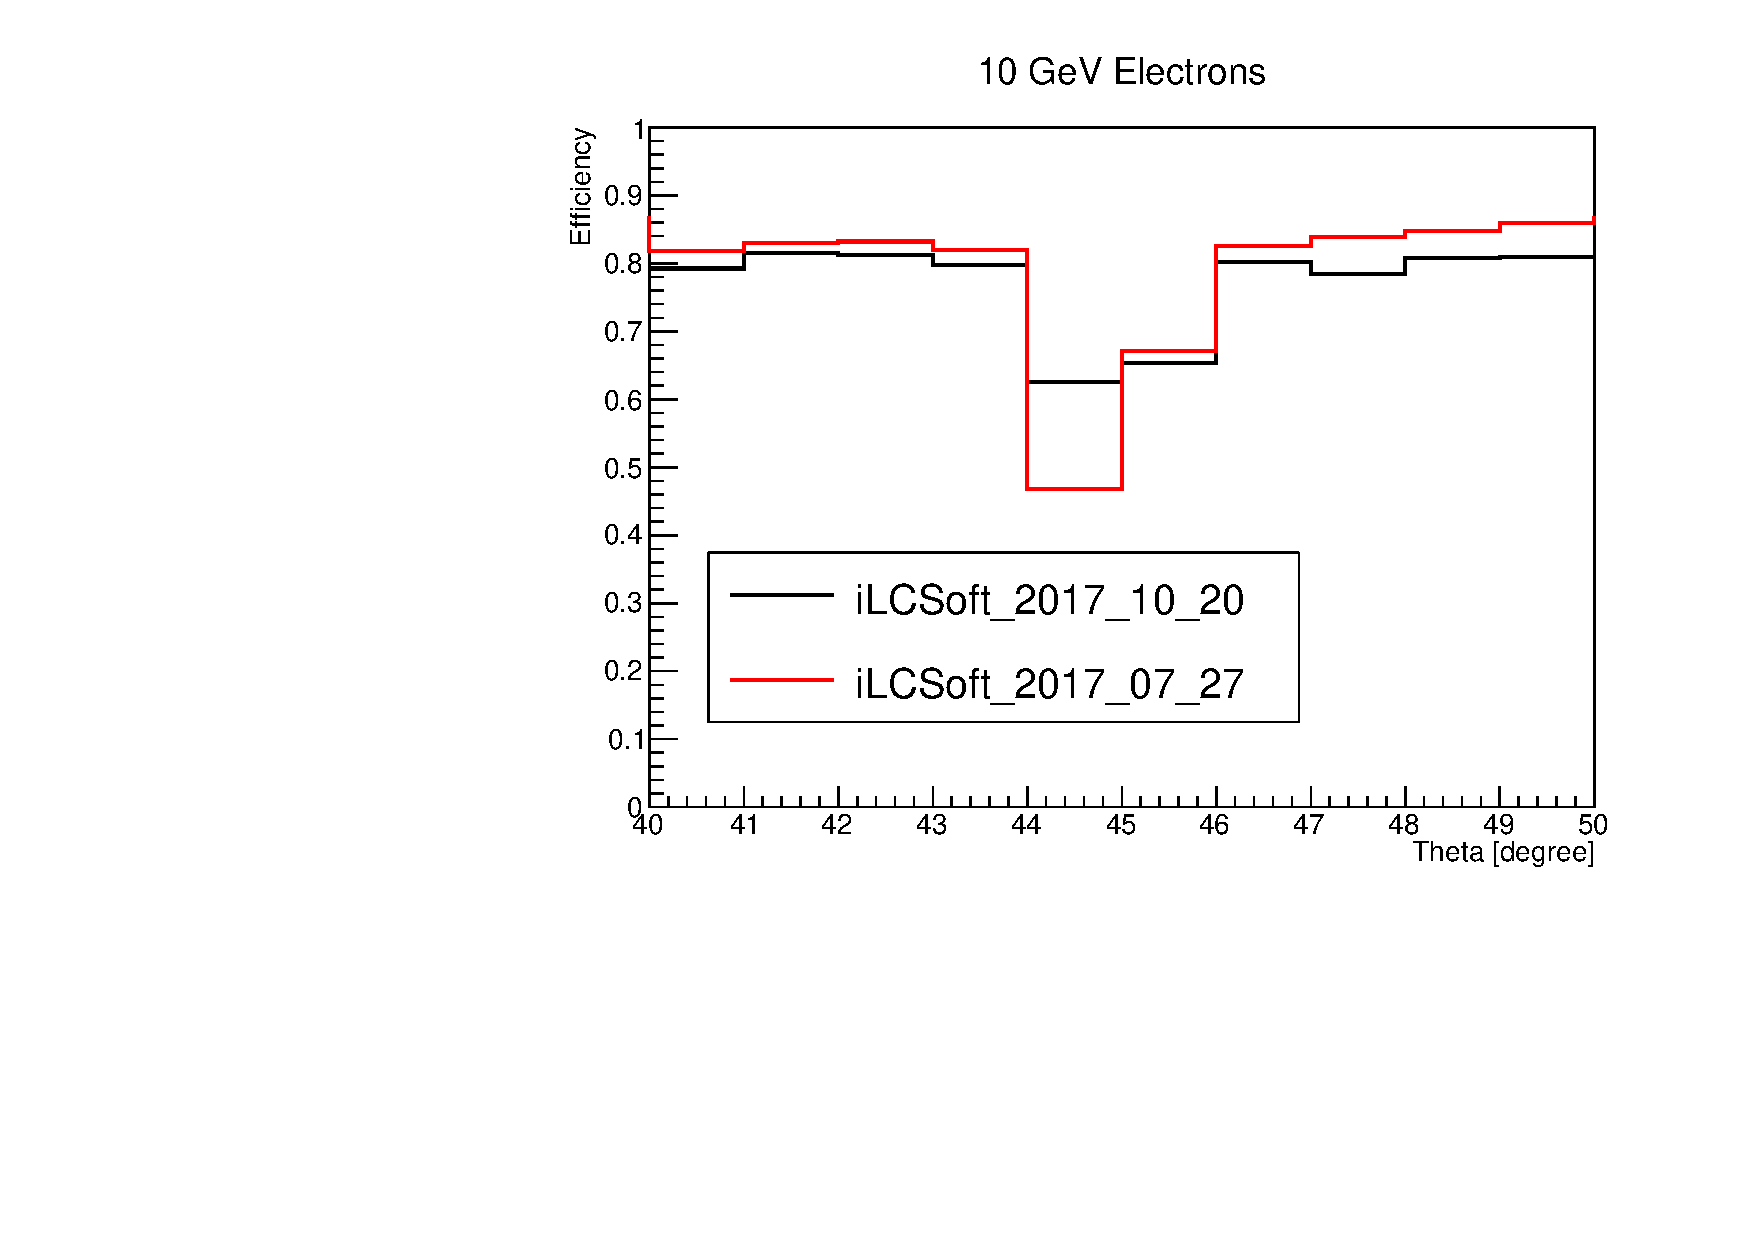
\includegraphics[width=6cm]{electrons_eff_vs_theta_zoomed.pdf}};
  \node [Box] at (\xRefPosOne+3,\yRefPosOne-0.7) (box){%
   \myCenterBox{10 GeV Electrons, transition region}
  };
      
%  \node[inner sep=0pt] (tmp) at (\xRefPosOne+3,\yRefPosOne-2.7)
%     {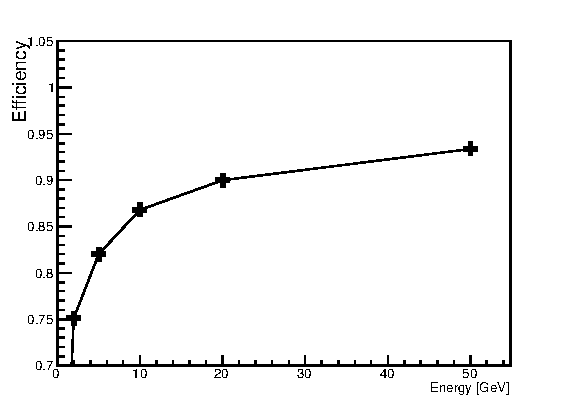
\includegraphics[width=6cm]{sep27/electron_eff.pdf}};



%% HELPER draw advanced helping grid with axises:
% \draw(-0.5,-4) to[grid with coordinates] (11.5,4);
\end{tikzpicture}
 
\end{frame}
%*****************************************************************************
%*****************************************************************************
\begin{frame}{\large \large Jet energy resolution FCC-ee vs. CLIC}
\renewcommand{\yRefPosOne}{0}
\renewcommand{\xRefPosOne}{5.3}
\renewcommand{\xRefIncrementOne}{5.5}
\begin{tikzpicture}[overlay]
 
 \node[inner sep=0pt] (tmp) at (\xRefPosOne-3,\yRefPosOne+0.7)
  {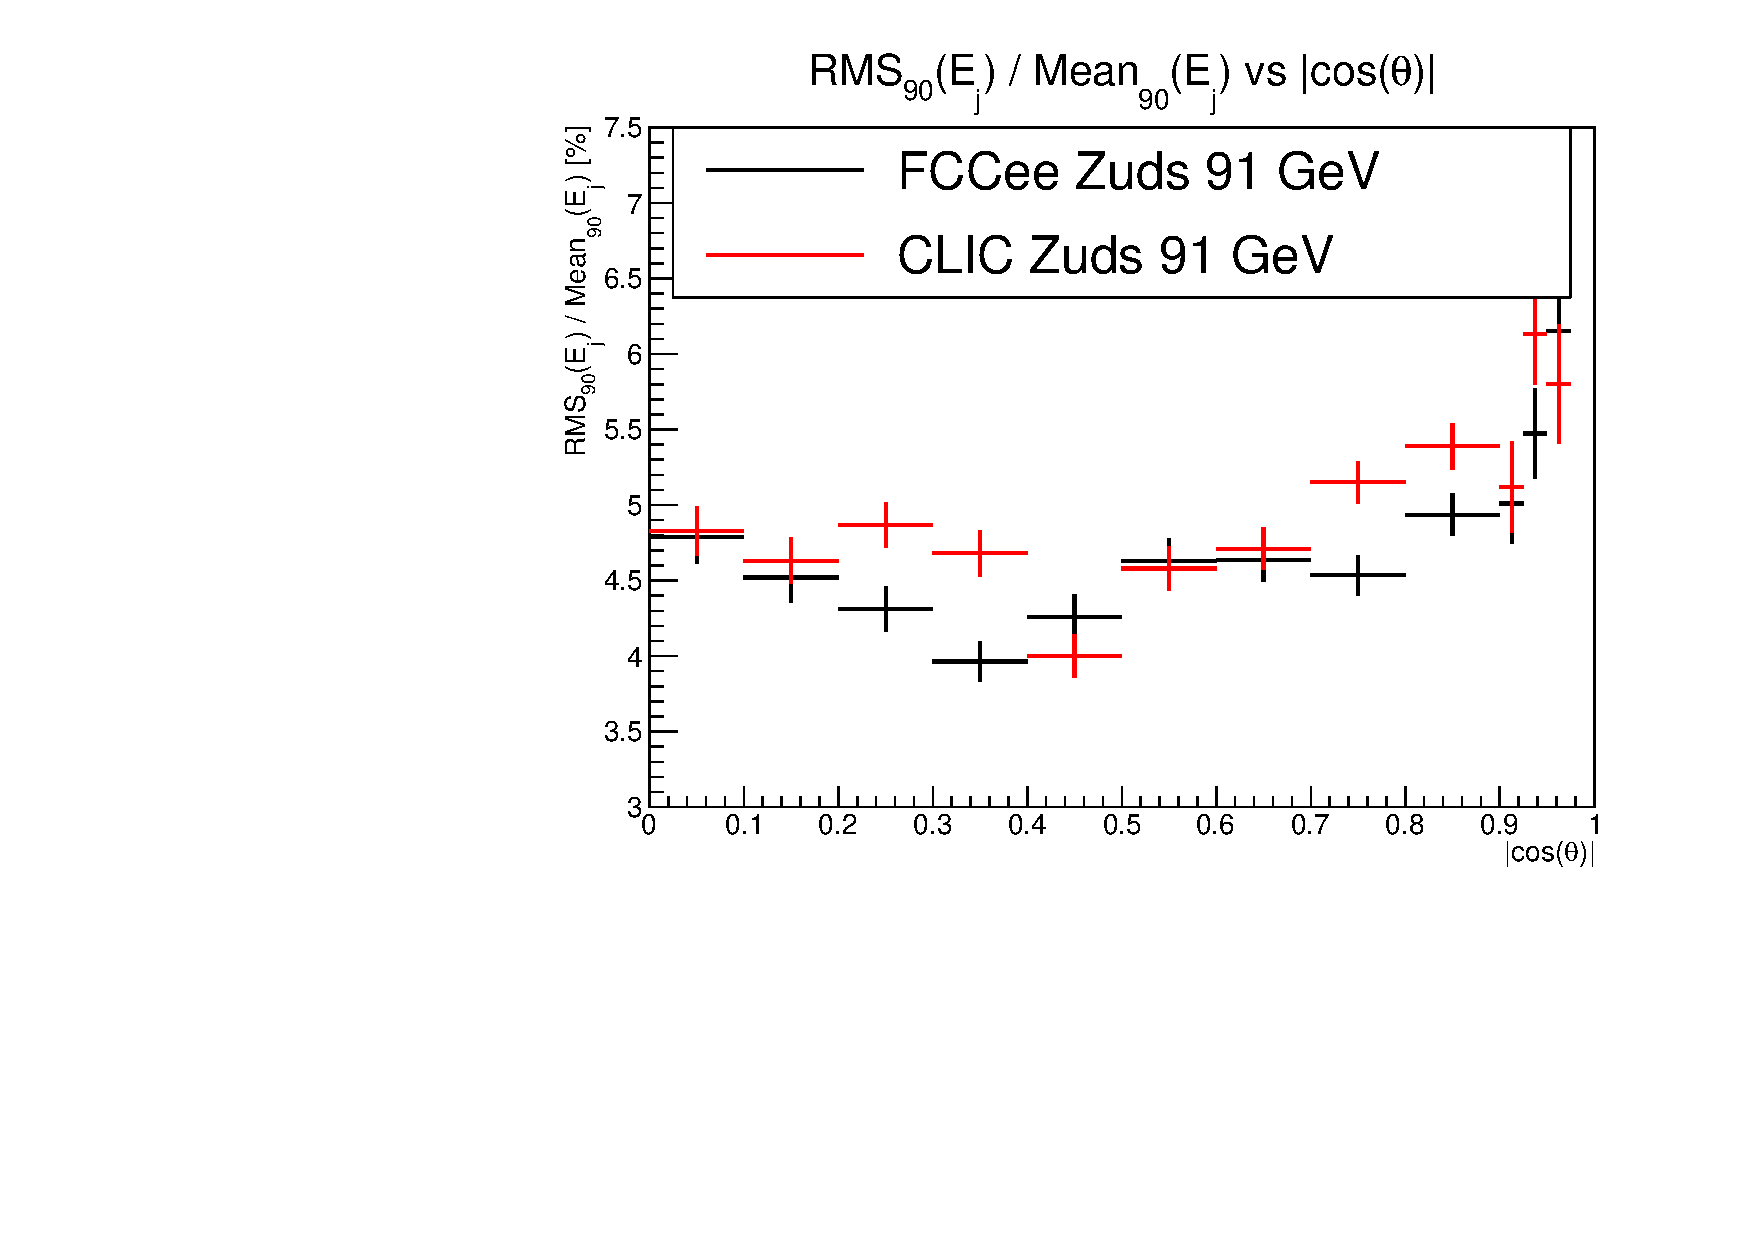
\includegraphics[width=6cm]{jet_eRes_FCCee_CLIC_91.pdf}};

  
  
 \node[inner sep=0pt] (tmp) at (\xRefPosOne+3,\yRefPosOne+0.7)
  {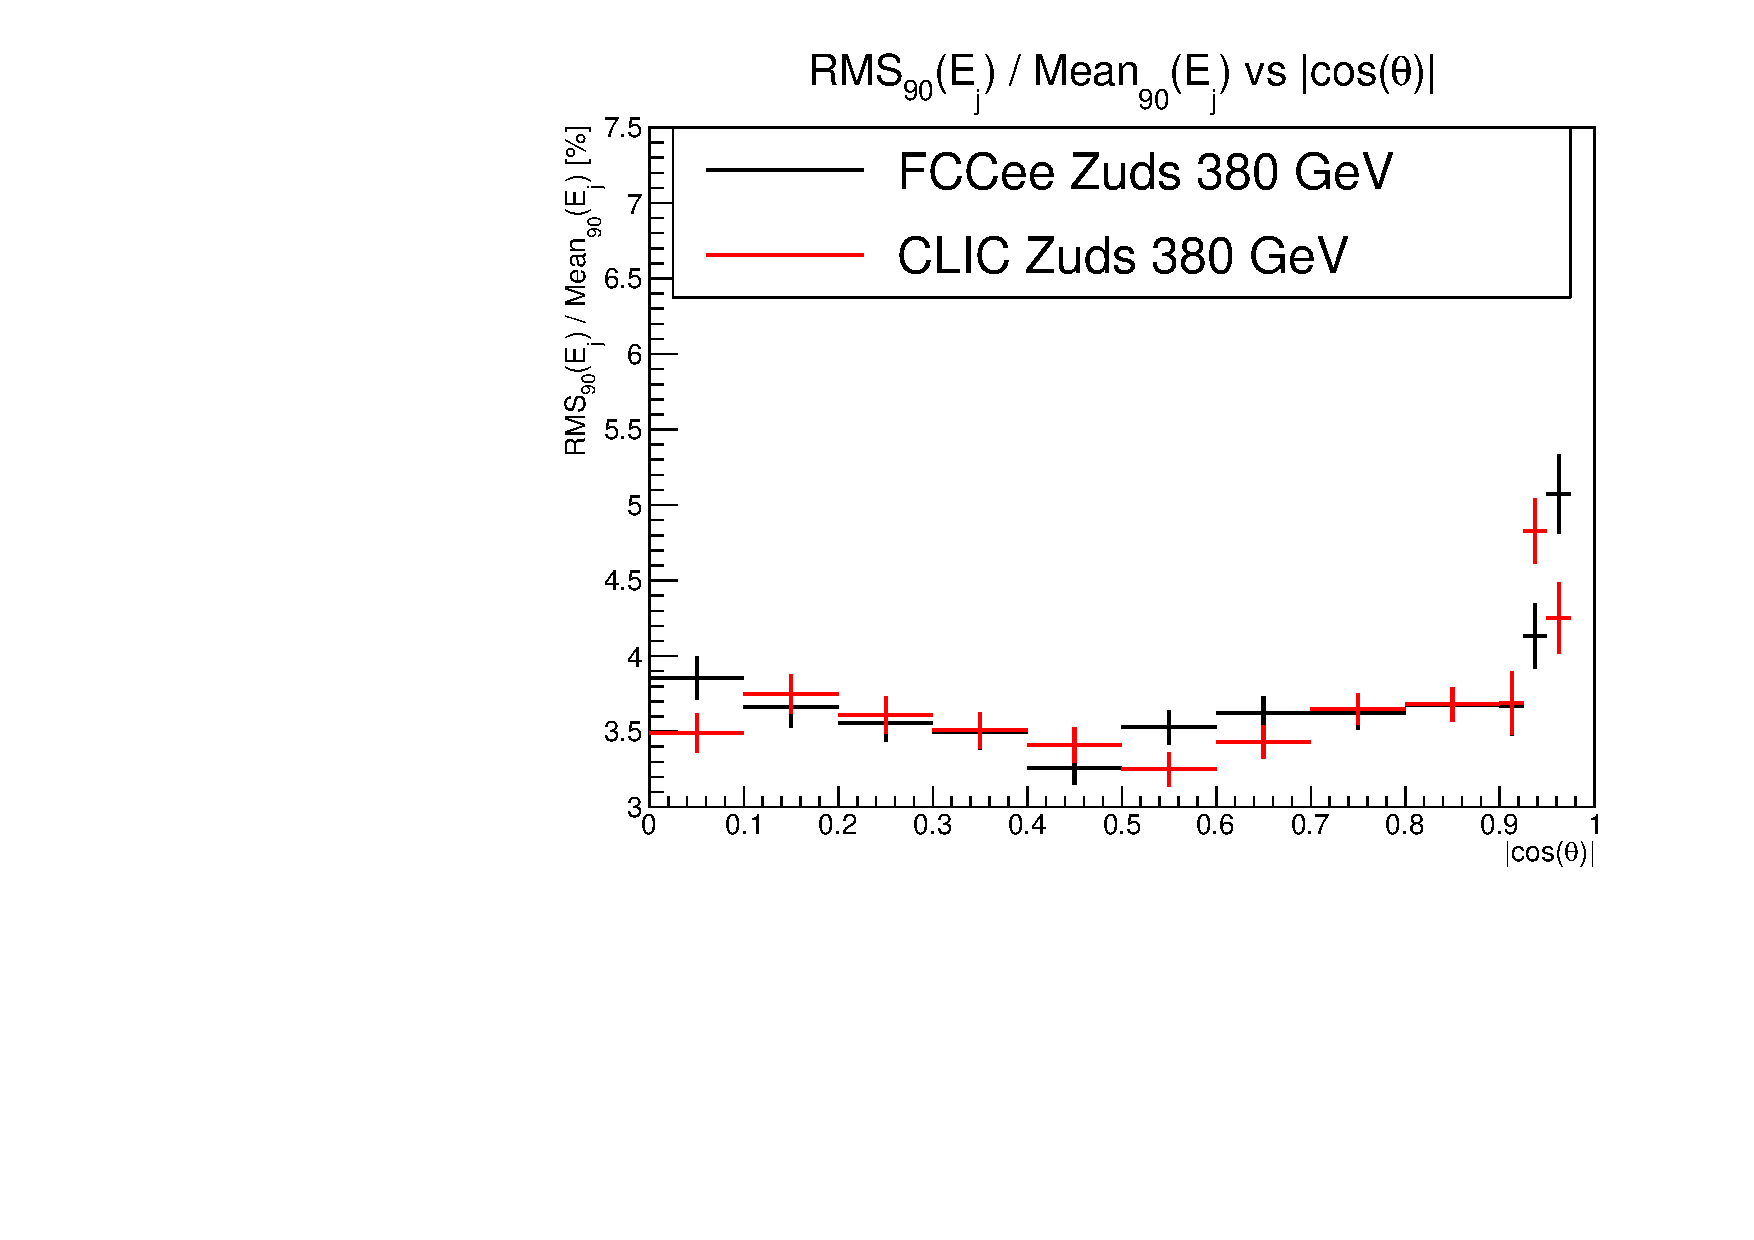
\includegraphics[width=6cm]{jet_eRes_FCCee_CLIC_380.pdf}};
  
% \node [PixelBox] at (\xRefPosOne-3,\yRefPosOne-2.5) (box){
%     \begin{minipage}{0.34\textwidth}
%     \hspace{0.9cm}$\sigma_{E}/ E \simeq$ 1.5 $\%$  
%     \\ reached for 100 GeV photons
%     \end{minipage}
% };

\node [Box] at (\xRefPosOne,\yRefPosOne-2.5) (box){%
    \begin{minipage}{\textwidth}
%        \scriptsize 
        \begin{itemize}
      \item Comparable jet resolution between FCC-ee and CLIC as expected
    \end{itemize}

    \end{minipage}
};
  
  
\end{tikzpicture}
\end{frame}
%*****************************************************************************


\end{document}

